
\documentclass[a4paper,11pt]{article}
\usepackage[a4paper, margin=8em]{geometry}

% usa i pacchetti per la scrittura in italiano
\usepackage[french,italian]{babel}
\usepackage[T1]{fontenc}
\usepackage[utf8]{inputenc}
\frenchspacing 

% usa i pacchetti per la formattazione matematica
\usepackage{amsmath, amssymb, amsthm, amsfonts}

% usa altri pacchetti
\usepackage{gensymb}
\usepackage{hyperref}
\usepackage{standalone}

\usepackage{colortbl}

\usepackage{xstring}
\usepackage{karnaugh-map}

% imposta il titolo
\title{Electronics for Embedded Systems notes}
\author{Luca Seggiani}
\date{2026}

% spaziatura liste
\usepackage{enumitem}
\setlist[itemize]{noitemsep, topsep=4pt, partopsep=0pt, parsep=2pt, leftmargin=*}
\setlist[enumerate]{noitemsep, topsep=4pt, partopsep=0pt, parsep=2pt, leftmargin=*}

% imposta lo stile
% usa helvetica
\usepackage[scaled]{helvet}
% usa palatino
\usepackage{palatino}
% usa un font monospazio guardabile
\usepackage{lmodern}

\renewcommand{\rmdefault}{ppl}
\renewcommand{\sfdefault}{phv}
\renewcommand{\ttdefault}{lmtt}

% circuiti
\usepackage{circuitikz}
\usetikzlibrary{babel}

% testo cerchiato
\newcommand*\circled[1]{\tikz[baseline=(char.base)]{
            \node[shape=circle,draw,inner sep=2pt] (char) {#1};}}

% disponi il titolo
\makeatletter
\renewcommand{\maketitle} {
	\begin{center} 
		\begin{minipage}[t]{.8\textwidth}
			\textsf{\huge\bfseries \@title} 
		\end{minipage}%
		\begin{minipage}[t]{.2\textwidth}
			\raggedleft \vspace{-1.65em}
			\textsf{\small \@author} \vfill
			\textsf{\small \@date}
		\end{minipage}
		\par
	\end{center}

	\thispagestyle{empty}
	\pagestyle{fancy}
}
\makeatother

% disponi teoremi
\usepackage{tcolorbox}
\newtcolorbox[auto counter, number within=section]{theorem}[2][]{%
	colback=blue!10, 
	colframe=blue!40!black, 
	sharp corners=northwest,
	fonttitle=\sffamily\bfseries, 
	title=Theorem~\thetcbcounter: #2, 
	#1
}

% disponi definizioni
\newtcolorbox[auto counter, number within=section]{definition}[2][]{%
	colback=red!10,
	colframe=red!40!black,
	sharp corners=northwest,
	fonttitle=\sffamily\bfseries,
	title=Definition~\thetcbcounter: #2,
	#1
}

% disponi codice
\usepackage{listings}
\usepackage[table]{xcolor}

\definecolor{codegreen}{rgb}{0,0.6,0}
\definecolor{codegray}{rgb}{0.5,0.5,0.5}
\definecolor{codepurple}{rgb}{0.58,0,0.82}
\definecolor{backcolour}{rgb}{0.95,0.95,0.92}

\lstdefinestyle{codestyle}{
		backgroundcolor=\color{black!5}, 
		commentstyle=\color{codegreen},
		keywordstyle=\bfseries\color{magenta},
		numberstyle=\sffamily\tiny\color{black!60},
		stringstyle=\color{green!50!black},
		basicstyle=\ttfamily\footnotesize,
		breakatwhitespace=false,         
		breaklines=true,                 
		captionpos=b,                    
		keepspaces=true,                 
		numbers=left,                    
		numbersep=5pt,                  
		showspaces=false,                
		showstringspaces=false,
		showtabs=false,                  
		tabsize=2
}

\lstdefinestyle{shellstyle}{
		backgroundcolor=\color{black!5}, 
		basicstyle=\ttfamily\footnotesize\color{black}, 
		commentstyle=\color{black}, 
		keywordstyle=\color{black},
		numberstyle=\color{black!5},
		stringstyle=\color{black}, 
		showspaces=false,
		showstringspaces=false, 
		showtabs=false, 
		tabsize=2, 
		numbers=none, 
		breaklines=true
}

\lstdefinelanguage{x86}{ 
  keywords={AAA, AAD, AAM, AAS, ADC, ADCB, ADCW, ADCL, ADD, ADDB, ADDW, ADDL, AND, ANDB, ANDW, ANDL,
        ARPL, BOUND, BSF, BSFL, BSFW, BSR, BSRL, BSRW, BSWAP, BT, BTC, BTCB, BTCW, BTCL, BTR, 
        BTRB, BTRW, BTRL, BTS, BTSB, BTSW, BTSL, CALL, CBW, CDQ, CLC, CLD, CLI, CLTS, CMC, CMP,
        CMPB, CMPW, CMPL, CMPS, CMPSB, CMPSD, CMPSW, CMPXCHG, CMPXCHGB, CMPXCHGW, CMPXCHGL,
        CMPXCHG8B, CPUID, CWDE, DAA, DAS, DEC, DECB, DECW, DECL, DIV, DIVB, DIVW, DIVL, ENTER,
        HLT, IDIV, IDIVB, IDIVW, IDIVL, IMUL, IMULB, IMULW, IMULL, IN, INB, INW, INL, INC, INCB,
        INCW, INCL, INS, INSB, INSD, INSW, INT, INT3, INTO, INVD, INVLPG, IRET, IRETD, JA, JAE,
        JB, JBE, JC, JCXZ, JE, JECXZ, JG, JGE, JL, JLE, JMP, JNA, JNAE, JNB, JNBE, JNC, JNE, JNG,
        JNGE, JNL, JNLE, JNO, JNP, JNS, JNZ, JO, JP, JPE, JPO, JS, JZ, LAHF, LAR, LCALL, LDS,
        LEA, LEAVE, LES, LFS, LGDT, LGS, LIDT, LMSW, LOCK, LODSB, LODSD, LODSW, LOOP, LOOPE,
        LOOPNE, LSL, LSS, LTR, MOV, MOVB, MOVW, MOVL, MOVSB, MOVSD, MOVSW, MOVSX, MOVSXB,
        MOVSXW, MOVSXL, MOVZX, MOVZXB, MOVZXW, MOVZXL, MUL, MULB, MULW, MULL, NEG, NEGB, NEGW,
        NEGL, NOP, NOT, NOTB, NOTW, NOTL, OR, ORB, ORW, ORL, OUT, OUTB, OUTW, OUTL, OUTSB, OUTSD,
        OUTSW, POP, POPL, POPW, POPB, POPA, POPAD, POPF, POPFD, PUSH, PUSHL, PUSHW, PUSHB, PUSHA, 
        RCLL, RCR, RCRB, RCRW, RCRL, RDMSR, RDPMC, RDTSC, REP, REPE, REPNE, RET, ROL, ROLB, ROLW,
        ROLL, ROR, RORB, RORW, RORL, SAHF, SAL, SALB, SALW, SALL, SAR, SARB, SARW, SARL, SBB,
        SBBB, SBBW, SBBL, SCASB, SCASD, SCASW, SETA, SETAE, SETB, SETBE, SETC, SETE, SETG, SETGE,
        SETL, SETLE, SETNA, SETNAE, SETNB, SETNBE, SETNC, SETNE, SETNG, SETNGE, SETNL, SETNLE,
        SETNO, SETNP, SETNS, SETNZ, SETO, SETP, SETPE, SETPO, SETS, SETZ, SGDT, SHL, SHLB, SHLW,
        SHLL, SHLD, SHR, SHRB, SHRW, SHRL, SHRD, SIDT, SLDT, SMSW, STC, STD, STI, STOSB, STOSD,
        STOSW, STR, SUB, SUBB, SUBW, SUBL, TEST, TESTB, TESTW, TESTL, VERR, VERW, WAIT, WBINVD,
        XADD, XADDB, XADDW, XADDL, XCHG, XCHGB, XCHGW, XCHGL, XLAT, XLATB, XOR, XORB, XORW, XORL},
  keywordstyle=\color{blue}\bfseries,
  ndkeywordstyle=\color{darkgray}\bfseries,
  identifierstyle=\color{black},
  sensitive=false,
  comment=[l]{\#},
  morecomment=[s]{/*}{*/},
  commentstyle=\color{purple}\ttfamily,
  stringstyle=\color{red}\ttfamily,
  morestring=[b]',
  morestring=[b]"
}

\lstdefinelanguage{riscv}{
  keywords={
    LUI, AUIPC,
    JAL, JALR,
    BEQ, BNE, BLT, BGE, BLTU, BGEU,
    LB, LH, LW, LBU, LHU, LD,
    SB, SH, SW, SD,
    ADDI, SLTI, SLTIU, XORI, ORI, ANDI,
    SLLI, SRLI, SRAI,
    ADD, SUB, SLL, SLT, SLTU, XOR, SRL, SRA, OR, AND,
    ADDIW, SLLIW, SRLIW, SRAIW,
    ADDW, SUBW, SLLW, SRLW, SRAW,
    MUL, MULH, MULHSU, MULHU, DIV, DIVU, REM, REMU,
    MULW, DIVW, DIVUW, REMW, REMUW,
    LR.W, SC.W, AMOSWAP.W, AMOADD.W, AMOXOR.W,
    AMOAND.W, AMOOR.W, AMOMIN.W, AMOMAX.W,
    AMOMINU.W, AMOMAXU.W,
    LR.D, SC.D, AMOSWAP.D, AMOADD.D, AMOXOR.D,
    AMOAND.D, AMOOR.D, AMOMIN.D, AMOMAX.D,
    AMOMINU.D, AMOMAXU.D,
    FLW, FSW,
    FMADD.S, FMSUB.S, FNMSUB.S, FNMADD.S,
    FADD.S, FSUB.S, FMUL.S, FDIV.S, FSQRT.S,
    FSGNJ.S, FSGNJN.S, FSGNJX.S,
    FMIN.S, FMAX.S,
    FCVT.W.S, FCVT.WU.S, FCVT.S.W, FCVT.S.WU,
    FMV.X.W, FMV.W.X,
    FEQ.S, FLT.S, FLE.S,
    FLD, FSD,
    FMADD.D, FMSUB.D, FNMSUB.D, FNMADD.D,
    FADD.D, FSUB.D, FMUL.D, FDIV.D, FSQRT.D,
    FSGNJ.D, FSGNJN.D, FSGNJX.D,
    FMIN.D, FMAX.D,
    FCVT.W.D, FCVT.WU.D, FCVT.D.W, FCVT.D.WU,
    FCVT.S.D, FCVT.D.S,
    FMV.X.D, FMV.D.X,
    FEQ.D, FLT.D, FLE.D,
    CSRRW, CSRRS, CSRRC,
    CSRRWI, CSRRSI, CSRRCI,
    FENCE.I,
    FENCE,
    ECALL, EBREAK,
    MRET, SRET, URET,
    WFI,
    SFENCE.VMA,
    NOP, LI, LA, MV,
    NOT, NEG, NEGW,
    SEQZ, SNEZ, SLTZ, SGTZ,
    BEQZ, BNEZ, BLEZ, BGEZ, BLTZ, BGTZ,
    BGT, BLE, BGTU, BLEU,
    J, JR, RET,
    CALL, TAIL,
    RDINSTRET, RDCYCLE, RDTIME,
    CSRR, CSRW, CSRS, CSRC,
    CSRWI, CSRSI, CSRCI
  },
  keywordstyle=\color{blue}\bfseries,
  ndkeywordstyle=\color{darkgray}\bfseries,
  identifierstyle=\color{black},
  sensitive=false,
  comment=[l]{\#},
  morecomment=[s]{/*}{*/},
  commentstyle=\color{purple}\ttfamily,
  stringstyle=\color{red}\ttfamily,
  morestring=[b]',
  morestring=[b]"
}

\lstdefinelanguage{arm}{
  keywords={
    ADC, ADD, AND, BIC, CMN, CMP, EOR, MOV, MVN,
    RSB, RSC, SBC, SUB, TST, TEQ,
    MLA, MLS, MUL, SMLAL, SMULL, UMLAL, UMULL,
    QADD, QSUB, QDADD, QDSUB,
    QADD16, QADD8, QASX, QSAX,
    QSUB16, QSUB8, QSAX, QSUBADDX,
    ASR, LSL, LSR, ROR, RRX,
    B, BL, BX, BLX,
    BXJ,
    BEQ, BNE, BCS, BHS, BCC, BLO,
    BMI, BPL, BVS, BVC,
    BHI, BLS, BGE, BLT, BGT, BLE,
    BAL,
    LDR, LDRB, LDRH, LDRSB, LDRSH,
    LDRD, LDM, LDMIA, LDMIB, LDMDA, LDMDB,
    LDRT, LDRBT, LDRHT, LDRSBT, LDRSHT,
    STR, STRB, STRH, STRD,
    STM, STMIA, STMIB, STMDA, STMDB,
    STRT, STRBT, STRHT,
    PUSH, POP,
    SWP, SWPB,
    REV, REV16, REVSH,
    BFC, BFI, BFXIL, SBFX, UBFX,
    CLZ,
    LDREX, LDREXB, LDREXH, LDREXD,
    STREX, STREXB, STREXH, STREXD,
    DMB, DSB, ISB,
    MCR, MCRR, MRC, MRRC,
    MRS, MSR,
    CPS, SETEND, SVC, BKPT,
    CLREX, WFE, WFI, SEV,
    YIELD, NOP,
    VLDR, VSTR,
    VMOV, VABS, VNEG,
    VADD, VSUB, VMUL, VDIV,
    VMLA, VMLS, VNMLA, VNMLS, VNMUL,
    VMAX, VMIN,
    VSQRT,
    VCMP, VCMPE,
    VCVT,
    VCLZ, VCLS,
    VAND, VORR, VEOR, VBIC, VMVN,
    VLD1, VLD2, VLD3, VLD4,
    VST1, VST2, VST3, VST4,
    ADR, ADCS, ADDS, SUBS, MOVS, ANDS, ORRS, EORS
  },
  keywordstyle=\color{blue}\bfseries,
  ndkeywordstyle=\color{darkgray}\bfseries,
  identifierstyle=\color{black},
  sensitive=false,
  comment=[l]{@},
  morecomment=[l]{;},
  morecomment=[s]{/*}{*/},
  commentstyle=\color{purple}\ttfamily,
  stringstyle=\color{red}\ttfamily,
  morestring=[b]',
  morestring=[b]"
}

\lstset{style=codestyle, language=C}

% disponi sezioni
\usepackage{titlesec}

\titleformat{\section}
	{\sffamily\Large\bfseries} 
	{\thesection}{1em}{} 
\titleformat{\subsection}
	{\sffamily\large\bfseries}   
	{\thesubsection}{1em}{} 
\titleformat{\subsubsection}
	{\sffamily\normalsize\bfseries} 
	{\thesubsubsection}{1em}{}

% tikz
\usepackage{tikz}

% float
\usepackage{float}

% grafici
\usepackage{pgfplots}
\pgfplotsset{width=10cm,compat=1.9}

% disponi alberi
\usepackage{forest}

\forestset{
	rectstyle/.style={
		for tree={rectangle,draw,font=\large\sffamily}
	},
	roundstyle/.style={
		for tree={circle,draw,font=\large}
	}
}

% disponi algoritmi
\usepackage{algorithm}
\usepackage{algorithmic}
\makeatletter
\renewcommand{\ALG@name}{Algorithm}
\makeatother

% disponi numeri di pagina
\usepackage{fancyhdr}
\fancyhf{} 
\fancyfoot[L]{\sffamily{\thepage}}

\makeatletter
\fancyhead[L]{\raisebox{1ex}[0pt][0pt]{\sffamily{\@title \ \@date}}} 
\fancyhead[R]{\raisebox{1ex}[0pt][0pt]{\sffamily{\@author}}}
\makeatother

\begin{document}
% sezione (data)
\section{Lesson 04-11-26}

% stili pagina
\thispagestyle{empty}
\pagestyle{fancy}

% testo
\subsection{CAN}

\textbf{CAN} (\textit{Controller Area Network}) is a protocol aimed to increase communication rate, and increase interconnect length.

Defined by Bosch in 1980, it supports a \textit{multi-node} topology, with multiple blocks on the same bus, and all blocks acting as masters (one-to-many with node arbitration).

It was developed for automotive applications, but also used in other contexts.
It's designed for noisy environments.

The protocols defines several aspects of the communication:
\begin{itemize}
	\item \textbf{Physical} (electrical) level
	\item \textbf{Transaction} (frame format) level
	\item \textbf{Software} (application) level
\end{itemize}

It is a serial communication with an embedded clock, which means it has a high clock frequency, not affected by skew (though it isn't suited to short interconnections).

Of course, it requires special encodings and circuits, such as clock decoders at the receiver, ro extract the clock information and the data stream.

As for increasing interconnection length, skew is very high for long interconnections, so we use a serial communication with embedded clock.

We also use \textit{differential signaling} to reduce the effects of noise.

\begin{center}
	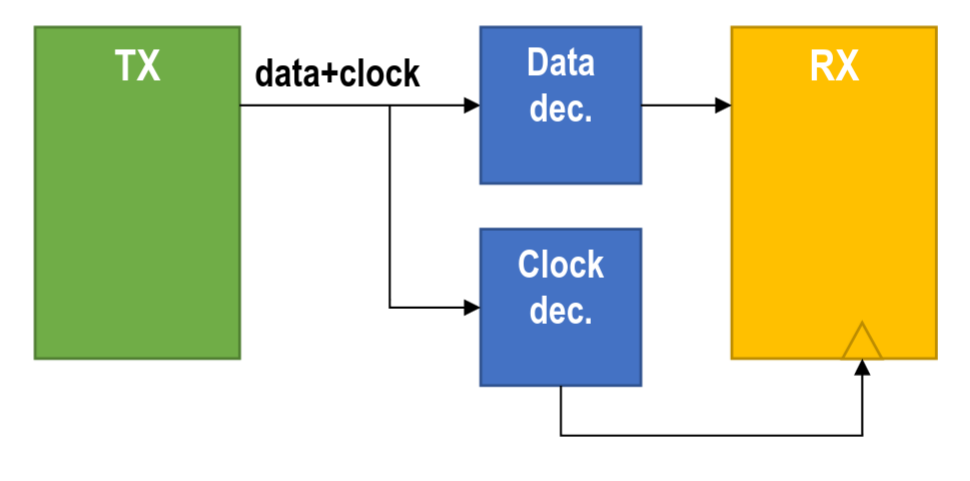
\includegraphics[scale=0.22]{../figures/can_base.png}
\end{center}

\subsubsection{Differential signaling}

Now, in a real communication system, if we transmit signals via 2 wires (data and ground), we never get exactly the same voltage at RX and TX $V^{TX} \neq V^{RX}$.
This is because of ground differences, making the ground not a good reference for the data line (which suffers from interference of its own).

\begin{center}
	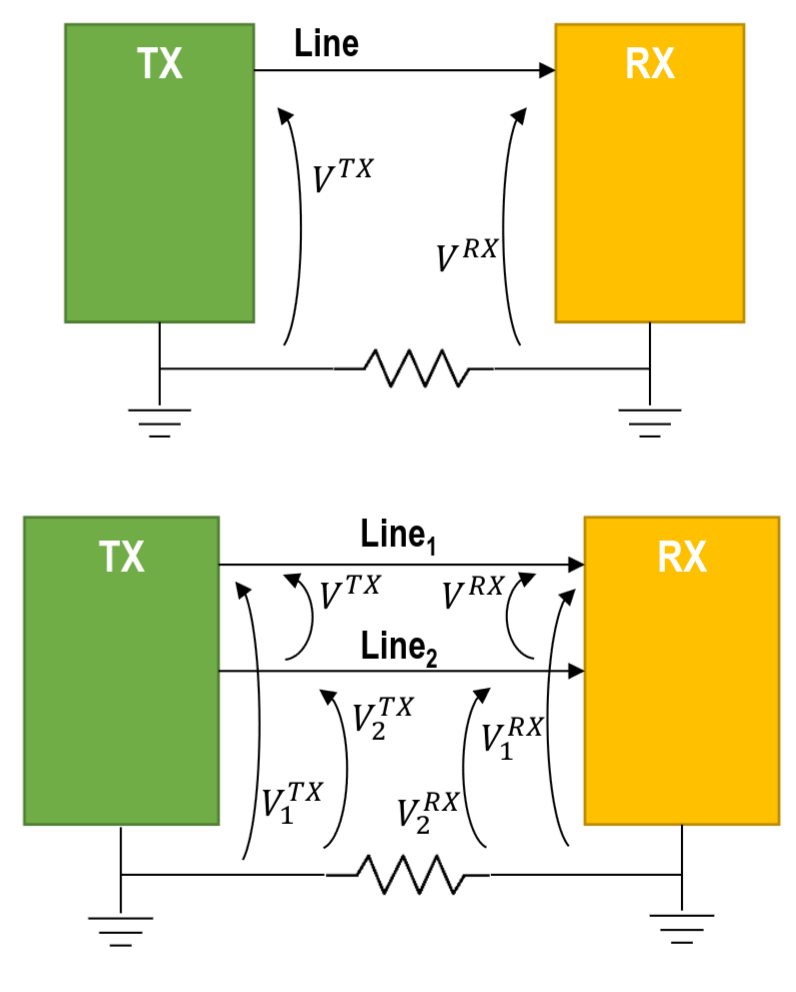
\includegraphics[scale=0.22]{../figures/can_diff.png}
\end{center}

What we do is encode information as the voltage difference between two wires.
Assuming $V_{CM}$ is equal to the difference between the two grounds, and interference carried on both the data wires (\textit{Common Mode Noise}, \textbf{CMD}), we have:
$$
V_1^{RX} = V_1^{TX} + V_{CM}, \quad V_2^{RX} = V_2^{®X} + V_{CM}
$$
And we can recover, via operational amplifiers at both ends:
$$
V^{RX} = V_1^{RX} - V_2^{RX} = V_1^{TX} + V_{CM} - V_2^{TX} - V_{CM} = V_1^{TX} - V_2^{TX} = V^{TX}
$$

This both RX and TX see the same voltage, whatever the ground differences, losses, and other interference.

\par\smallskip

Let's focus on what we mean by interference: any other unwanted interference that equally affects both wires induces \textit{common mode noise}, which is cancelled by differential signaling.

This means we don't want wires affected by different noise (\textit{differential mode nosie}), that is noise source close to one wire, for instance.

To aid in this, we \textit{twist} the pair of wires so that the interference alternatively affects one wire and the other.
Assuming the interference is uniform along multiple twists, the noise becomes common mode, and is cancelled by differential signaling.
We can also \textit{shield} the pair to reject interferences.

This gives a reason behind the wires we are used to:
\begin{itemize}
	\item \textbf{STP} (\textit{Shielded Twisted Pair});
	\item \textbf{UTP} (\textit{Unshielded Twisted Pair}).
\end{itemize}

\begin{center}
	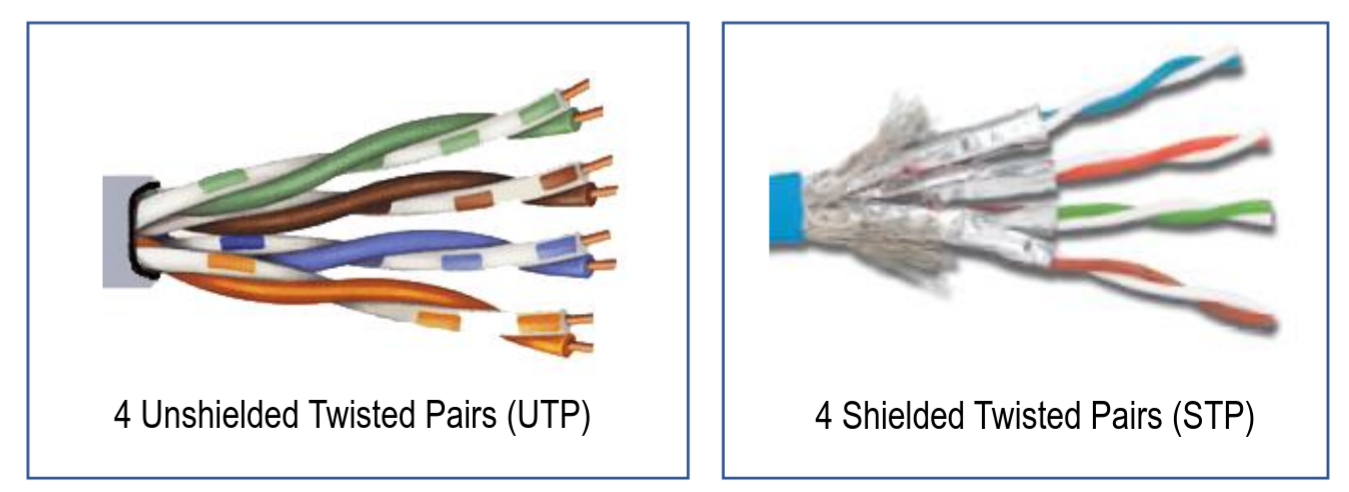
\includegraphics[scale=0.22]{../figures/stp_utp.png}
\end{center}

\par\smallskip

So, we have that the CAN protocol does differential signaling on two wires: \textbf{CANH} and \textbf{CANL}.

The two wires are used for data transfer, not one for data and the other for clock, like in I2C: there is no dedicated wire for the clock, so we don't suffer the problem of skew.

Data is in fact encoded as the difference CANH - CANL, which allows for long interconnections through embedded clock encoding.
The clock is recovered from data.

\par\smallskip

Let's look at the CAN bus itself.

\begin{center}
	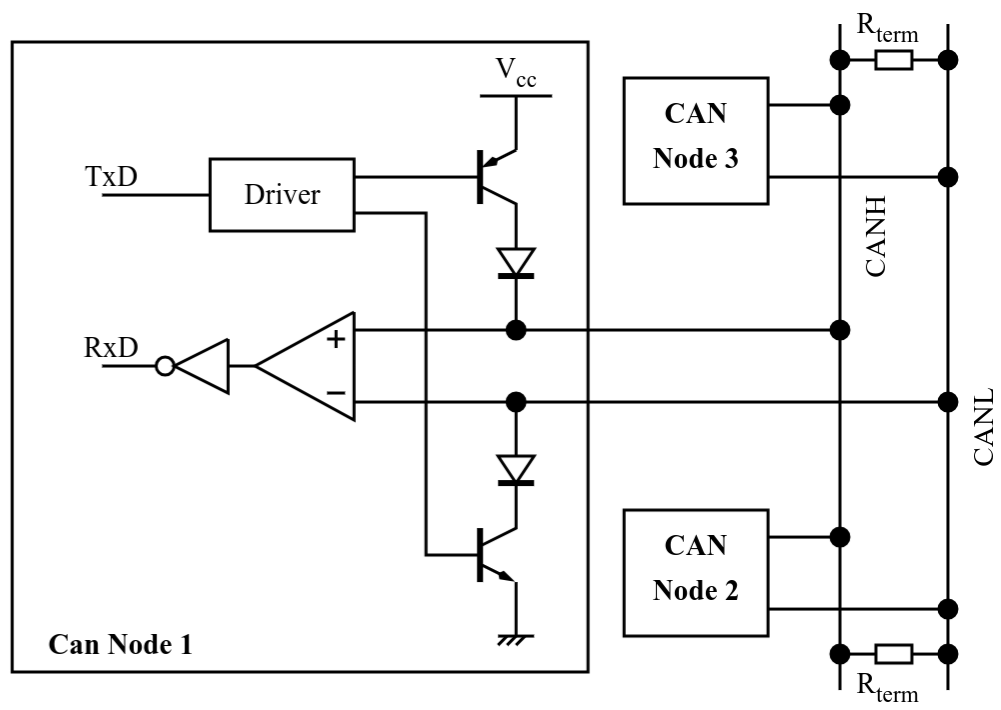
\includegraphics[scale=0.22]{../figures/can_bus.png}
\end{center}

We notice open collector driving of CANH and CANL, driving on the high side (through a PNP) for CANH, and on the low side (through an NPN) for CANL.
Reading, as we said, is done through a differential amplifier $V_{out} = CANH - CANL$, with an invertd output.

We have a terminating resistances between CANH and CANL, with value $120 \, \Omega$, meaning the resistance between the two CAN lines is $60 \, \Omega$.
This resistance is used to equalize the two wires voltage values when floating, and used to avoid reflections on the transmission line, especially for long interconnections.

If each side of the can bus can only be driven in one direction (through open collector signaling), we wonder how logic levels are represented.
To solve this, we use a system that distinguishes floating (\textit{recessive}) values from driven ones:
\begin{itemize}
	\item \textbf{Logic 0} (\textit{dominant}): $CANH=5\,\mathrm{V}$, $CANL=0\,\mathrm{V}$, difference in reading is high, output of the input amplifier is low;
	\item \textbf{Logic 1} (\textit{recessive}): $CANH=HiZ$, $CANL=HiZ$, difference in reading is 0 (because of the equalizing resistance), output of the input amplifier is high.
\end{itemize}

\begin{center}
	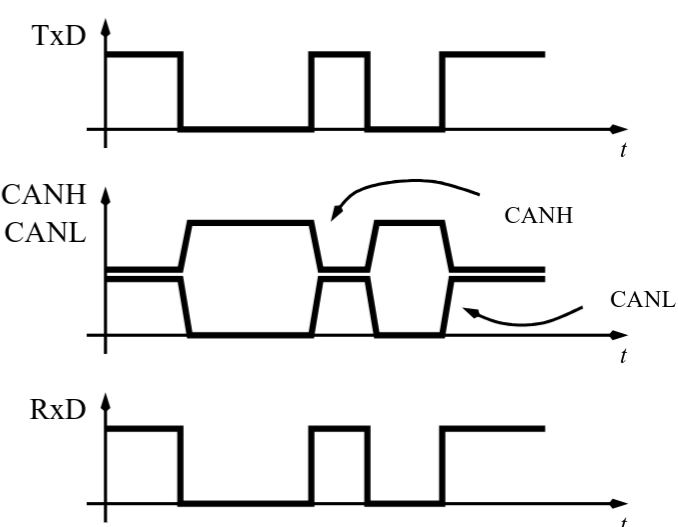
\includegraphics[scale=0.26]{../figures/can_sign.png}
\end{center}

Let's talk about bus contention: all nodes have the same interface on the CAN bus.
When not transmitting, each node generates a recessive bit, so a high value on receiver, and CANH and CANL are floating.
A dominant bit during transmission always wins over a recessive bit, as it means some node is driving the lines.
Since each node drives the lines to the same values on a dominant bit (open collector driving), in case of bus contention there are no damages or short circuits.

\par\smallskip

Since we said that NRZ encoding is used, with no guaranteed transitions we do bit stuffing after 5 consecutive identical bits:
\begin{itemize}
	\item After 5 dominant (0), insert a recessive (1);
	\item After 5 recessive (1), insert a dominant (0).
\end{itemize}
If 5 consecutive identical bits are followed by the opposite value, bit stuffing is applied anyway, so that the receiver can delete stuffed bits when decoding the incoming bitstream.

\par\smallskip

The eye diagram sees the bit time divided into 4 time quanta (8 to 25):
\begin{itemize}
	\item Synch segment
	\item Propagation segment
	\item Phase segment 1
	\item Phase segment 2
\end{itemize}
Sampling is specified to happen between Phase1 and Phase2 segments.

\begin{center}
	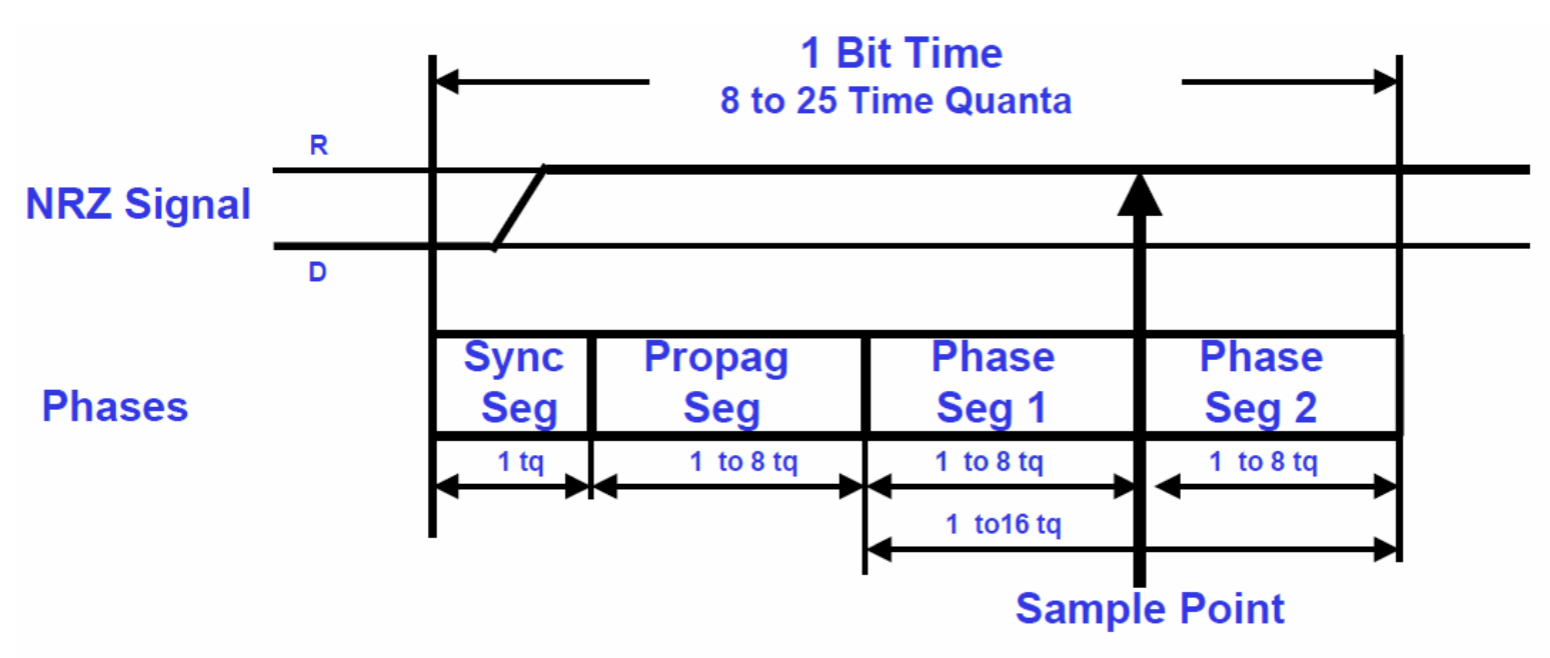
\includegraphics[scale=0.22]{../figures/can_eye.png}
\end{center}

\subsubsection{I2C protocol}

Enough electronics. Let's talk about the protocol.

Three main problems:
\begin{itemize}
\item \textbf{Synchronization}: all devices have to be synchronized at each recessive to dominant transition, with transitions assumed to happen at the beginning of a bit time. Each device momentarily adjusts Phase1 and Phase2 lengths to synch.
All devices start in low speed, and speed can be modified later at run-time;
\item \textbf{Addressing}: when transmitting, each node generates an 11 bit address, known as identifier in CAN. It is \textit{not} the address of the destination node;
\item \textbf{Arbitration}: similar to I2C, the lower identifier wins contention (dominant vs. recessive), as lower identifier means higher priority.
\end{itemize}

\begin{center}
	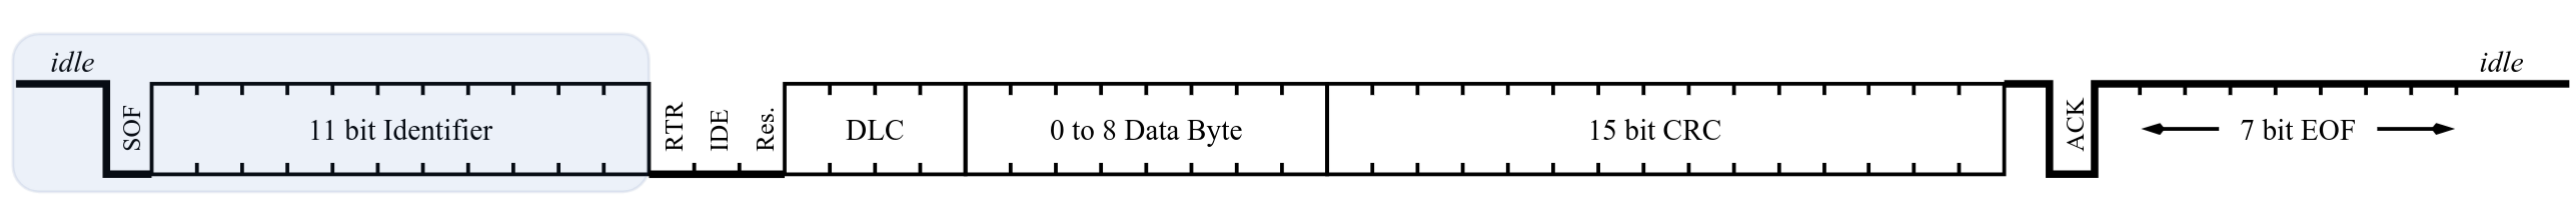
\includegraphics[scale=0.16]{../figures/can_protocol.png}
\end{center}

Let's see the full transmission in pratice.
\begin{enumerate}
	\item At idle, we see a recessive bit on the bus;
	\item \textit{Start Of Frame} (\textbf{SOF}) is a dominant bit generated by a node. It guarantees a recessive to dominant transition from the idle state. All other nodes synchronize their own clock, and avoid transmitting until the end of the frame;
	\item Then the \textit{identifier} is transmitted, on 11 bits (possibly extended to 29 through IDE);
	\item The \textit{Remote Transmission Request} (\textbf{RTR}) follows. 

		If a node wants to transmit data to other nodes, it is dominant to signal for data frames. 

		If a node requires data from another node it is recessive and the DLC indicates the number of requested bytes of data. Of course in this last case there is no data field.
	\item As we said, there's an \textbf{IDE} (\textit{ID Extension}) mode, flagged by the IDE bit (dominant for 11 bits);
	\item A reserved dominant bit is included in this flagging section;
	\item The \textit{Data Length Code} (\textbf{DLC}) follows, including the number of subsequent data bytes. It's a field on 4 bits, with acceptable values 0 to 8;
	\item We can finally transmit data. The \textit{data} field is 0 to 8 bytes (depends on DLC, 0 to 64 bits), but always a multiple of 8 bits;
	\item A \textit{Cyclic Redundancy Code} (\textbf{CRC}) is performed on 15 bits. One recessive bit flags the end of it;
	\item There's an acknowledge (\textbf{ACK}) bit: transmitter generates recessive, receivers generate dominant. This is also delimited by a recessive bit;
	\item Then we have the \textit{End Of Frame} (\textbf{EOF}), given by 7 consecutive bits, all recessive. Note that this is an intentional violation of the bit stuffing rule: bit stuffing is otherwise applied to all fields, except CRC delimiter, ACK and EOF.
	\item Now the bus returns idle, that is the always recessive. Other nodes can now start a transmission. Good for them.
\end{enumerate}

Notice that CAN defines higher protocol levels.
At the electrical level, all nodes on the bus are masters: any node can start a transmission, at any given time.
Arbitration on identifiers used to manage priorities and reception masks.

At higher levels of the protocol, some node have additional tasks: for instance to configure the bus and the other nodes, change the communication speed...
Just to summarize, several different higher level protocols can be dfined on top of the CAN physical layer.

\subsection{USB}

We all know \textbf{USB} (\textit{Universal Serial Bus}).
It was designed to substitute several kind of legacy connections, such as PS/2, RS232, ...
It supports Hot Plug\&Play, and different speeds (three in USB 2.0).

\begin{center}
	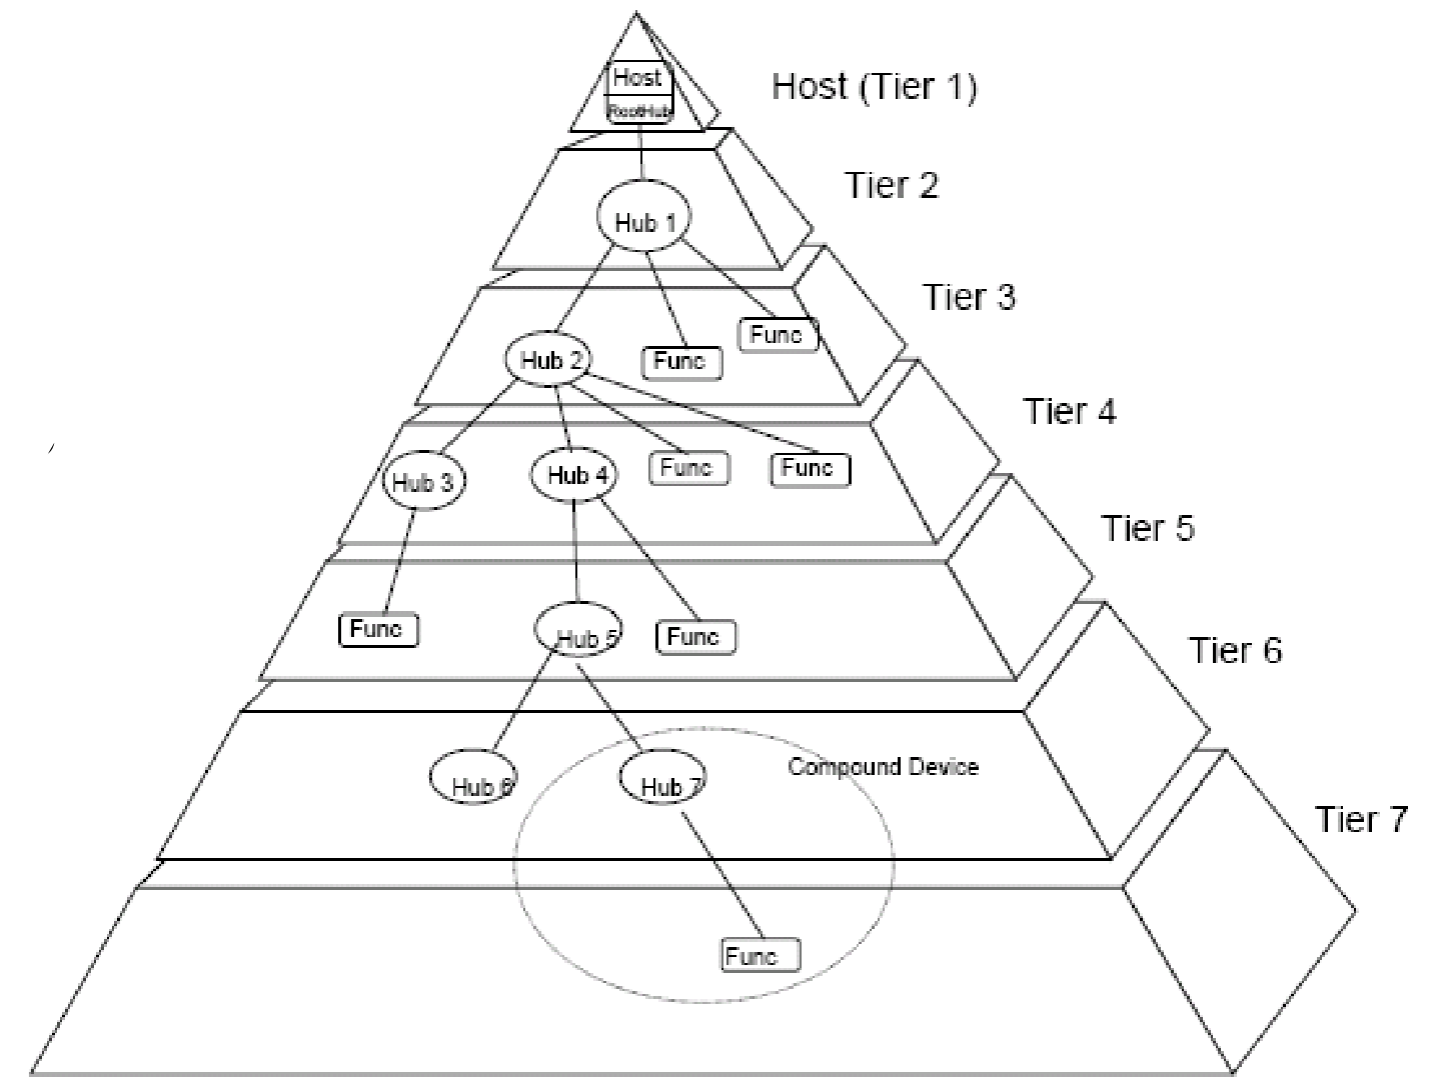
\includegraphics[scale=0.22]{../figures/usb_pyramid.png}
\end{center}

The USB Network has a tree structure: there's a single master (known as the \textit{host}), and up to 127 slaves (known as \textit{functions} or \textit{devices}), organized on up to 7 levels.
Always point-to-point communication between the single master and a slave; \textit{hubs} virtualize connections.

Since the USB Protocol defines a single master, there's no need for arbitration.
Each function (FUN) is assigned a unique address between 1 e 127, assigned when it is initially plugged in to the network.
Each FUN provides a maximum of 32 (16+16) end-points, with indexes 0 to 15.
For each index, there can be an end-point for reading, and another for writing.
Each end-point is unidirectional, with end-point 0 being always present

The USB standard is huge. It defines the behavior at several abstraction levels:
\begin{itemize}
\item Mechanical
\item Electrical
\item Protocol
\item Transactions
\item Multiple transfers
\item Driver
\item Application and managing software
\end{itemize}

\par\smallskip

The \textit{mechanical} standard is based on 4 wires, two for power:
\begin{itemize}
	\item $V_{BUS}$ at $5 \, \mathrm{V}$, $500 \, \mathrm{mA}$;
	\item The ground wire.
\end{itemize}

And a differential pair for data: $D^+$ and $D^-$ on STP.

\begin{center}
	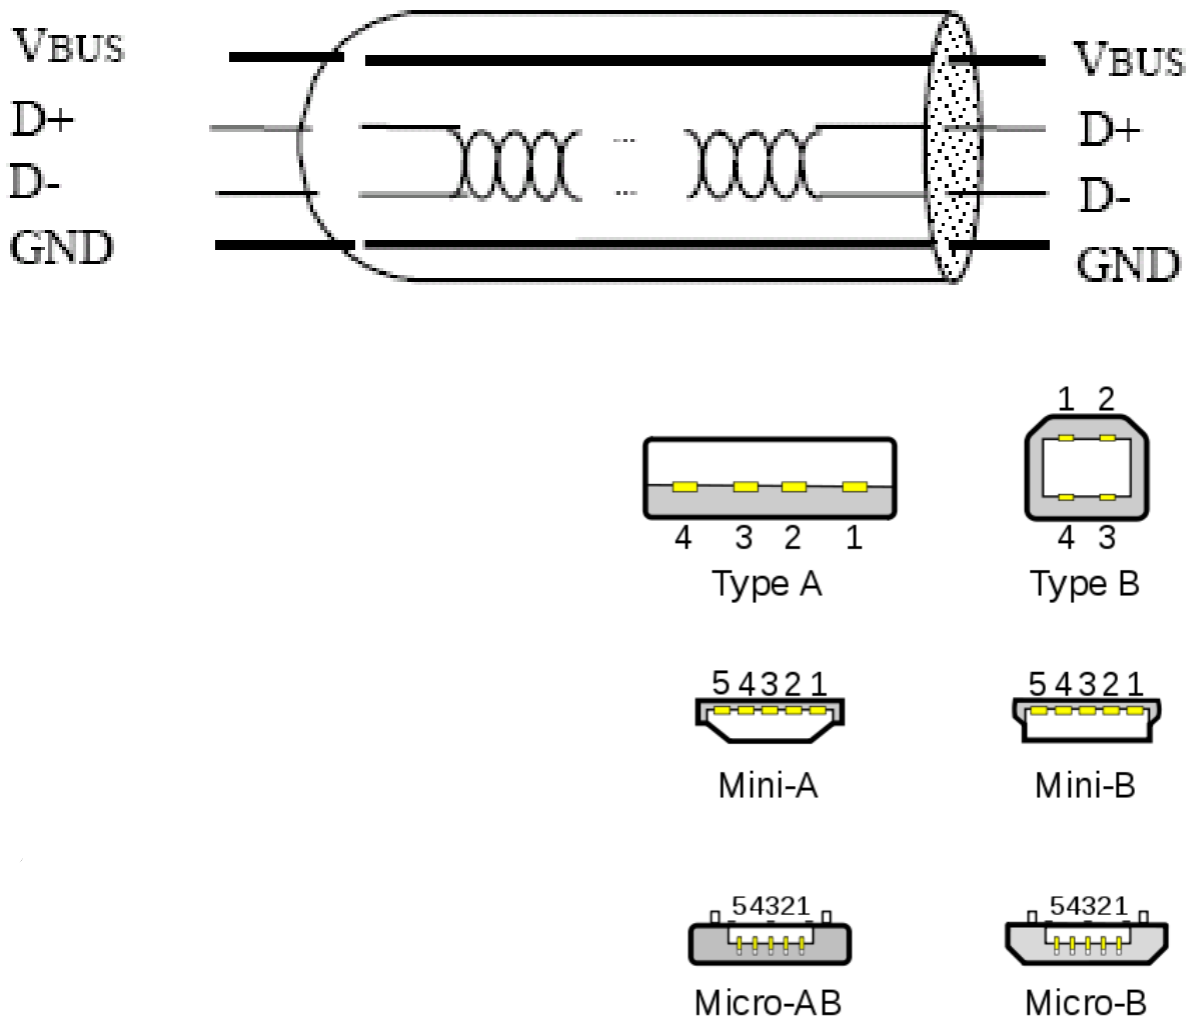
\includegraphics[scale=0.22]{../figures/usb_phys.png}
\end{center}

There are several kinds of physical connectors, that can be different between host and function.

\par\smallskip

USB does full differential signaling, with different voltage levels according to standard and speed configuration.
It features error checking and NRZI coding:
\begin{itemize}
\item \textbf{Logic 0}: transition (at the beginning of a bit);
\item \textbf{Logic 1}: maintains previous value.
\end{itemize}

\subsubsection{USB pipes}

At the \textit{transaction} level, communication on USB based on \textbf{pipes} (logical channels).
A pipe can be of stream or message type:
\begin{itemize}
\item Stream pipe:
\begin{itemize}
\item \textbf{Isochronous}: guaranteed bandwidth, possibly loosing data (audio, video, ...);
\item \textbf{Interrupt}: quick answer and guaranteed latency (keyboard, mouse, ...);
\item \textbf{Bulk}: large sporadic transfers, served using a best-effort bandwidth (file transfers, ...).
\end{itemize}
\item Message pipe:
\begin{itemize}
	\item \textbf{Control}: short commands to devices and status messages (configuration on end-point 0, ...).
\end{itemize}
\end{itemize}

\end{document}
